\documentclass[10pt, letterpaper]{article}
\usepackage [english]{babel}
\usepackage{enumitem}
\usepackage{geometry}
\usepackage{color}
\usepackage{tikz}
\usetikzlibrary{snakes}
\usetikzlibrary{patterns}
\usepackage{hyperref}

\newcommand{\todo}[1]{\textcolor{red}{TODO: #1}}

\geometry{margin=4cm}

\title{Rootkit of gruppe 6}
\author{Roman Karlstetter \and Philipp M\"uller}
\date{\today}

\begin{document}

\maketitle

\section{Overview}

This rootkit implements several functions, that can -- independently of each other -- be turned on and off. They are outlined here:

\begin{description}
\item [File hiding] It is possible to prevent some files to be shown. Files beginning with a certain prefix are hidden from e.g. \texttt{ls}. However, these files stay accessible.
\item [Process hiding] It is possible to hide certain processes by their ID.
\item [Module hiding] It is possible to hide the rootkit module from \texttt{lsmod}.
\item [Socket hiding] The rootkit can hide certain TCP and UDP sockets from \texttt{netstat} and \texttt{ss}.
\item [Privilege escalation] You can acquire the privileges to act as root.
\item [Covert communication] All this functionality is turned on and off via a covert communication channel.
\end{description}

\section{Building \& Installing}
You need to have a working environment for developing kernel modules. When this is the case, \texttt{cd} to the directory with the sources and execute \texttt{make} to build the module. This will create a file called \texttt{cool\_mod.ko}, which contains the compiled module.

\section{Usage}

\subsection{Loading the module}

The module is loaded like (probably) most other modules: using \texttt{insmod}. That is, you can just do the following:

\begin{verbatim}
root@machine:/path/to/rootkit# insmod cool_mod.ko
\end{verbatim}

Then, the module can be used. The module itself does quite a bit of output for the user, which can be used using \texttt{dmesg}. If you try \texttt{dmesg | tail -n 1} directly after loading, something like the following should be shown:

\begin{verbatim}
[   108.693480]  This is the kernel module of gruppe 6.
\end{verbatim}

\subsection{Using the module}

Once the module is loaded, it can receive commands as you type them into a shell. Every command starts with the prefix \texttt{\#\#\# } (three hashes, followed by one space).

Once this sequence of characters is entered, the rootkit expects the actual command. After the actual command, there might be a parameter (separated by a space from the command). Thus, the general format for commands is simply as follows:

\begin{verbatim}
### command params
\end{verbatim}

Where \texttt{command} is one of the following:

\begin{description}[font=\ttfamily]
\item[hideproc] This command expects a parameter representing the process ID of the process to be hidden. Hides the corresponding process.
\item[unhideproc] This command expects a parameter representing the process ID of the process to be unhidden. Unhides the corresponding process.
\item[hidemodule] Prevents the module from being shown when executing \texttt{lsmod}. Note that when the module is hidden, it can not be unloaded.
\item[unhidemodule] Unhides the module, i.e. \texttt{lsmod} is finding the module.
\item[hidetcp] Hides a TCP socket from \texttt{netstat} and \texttt{ss}. Expects one argument: The port of the socket to be hidden. 

Note that only one socket is hidden at a time, i.e. that if you call \texttt{hidetcp} twice, the first hiding will be discarded.
\item[hideudp] Hides a UDP socket from \texttt{netstat} and \texttt{ss}. Expects one argument: The port of the socket to be hidden.
\item[unhidesocket] Disables socket hiding.
\item[hidefiles] Hides files, whose filename is starting with \texttt{rootkit\_}, i.e. these files are ``invisible'' to \texttt{ls}, but can still be accessed.
\item[unhidefiles] Disables file hiding. I.e. basically all files are shown then (except those that are hidden by another rootkit ;) ).
\item[escalate] This command is most useful when invoked by a non-root-user. Once the module is loaded, \emph{any} user can just type \texttt{\#\#\# escalate} and obtains \texttt{root}-rights.
\end{description}

As an example, consider how to hide TCP socket 1234:

\begin{verbatim}
root@machine:/path/to/something# ### hidetcp 1234
\end{verbatim}

Note that you don't need to confirm the command by pressing return. The rootkit recognizes it as you type.

\section{Implementation Details}

We have split up things in header in implementation files, so
that our files don't get too large. The file names should be self-explanatory, but we should mention some things explicitly:

The files \texttt{sysmap.h} and \texttt{sysmap.c} are generated automatically by the script \texttt{create\_sysmap.h}. This script scans the ``system map'' of Linux (which is where all important function pointers to system call functions and other system functions are stored). All these pointers are collected and made usable to our code. The script prepends each found pointer with the prefix \texttt{ptr\_}. So, if you encounter a variable starting with this prefix, chances are good that it is something from the system map.

Note that all these pointers are of type \texttt{void*}, since we do not know their type a priori. They are later casted as needed.

\subsection{``Hooking'' functions in general}

A very important aspect of a rootkit is hooking of functions. This means, we ``grab'' an original system function (which may be called by other programs!), and replace it by our own function. This way, everytime another program tries to call the original function, it automatically calls \emph{our} ``injected'' function. Of course, the injected function should behave as if it was the original function, so that the other programs (and, thus, the user) do not recognize that we have manipulated the system function.

So, how is this hooking done programmatically? Let us consider how we hook the \texttt{read} system call, for example. This is done by the following code snippet\footnote{This is not the original source code of the rootkit, but just an excerpt of this function.}:

\begin{verbatim}
void hook_read(fun_void_charp_int cb){
    void** sys_call_table = (void *) ptr_sys_call_table;
    original_read = sys_call_table[__NR_read];
    make_page_writable((long unsigned int) ptr_sys_call_table);
    sys_call_table[__NR_read] = (void*) hooked_read;
    make_page_readonly((long unsigned int) ptr_sys_call_table);
}
\end{verbatim}

Let us consider this function line by line. First, we locate the system call table, which is basically just an array of pointers to system call functions. Afterwards, we retrieve the pointer to the original \texttt{read} system call and store it in  \texttt{original\_read}\footnote{\texttt{original\_read} is a function pointer of type \todo{which type???}}. This is necessary for several reasons: First, we want to be able to restore the original call if we want to unload the module. Moreover, as we will see later, we delegate the work to the original \texttt{read} function and just do some manipulations beforehand.

Let us -- for now -- skip the next line and directly consider the following line from the above snippet:

\begin{verbatim}
    sys_call_table[__NR_read] = (void*) hooked_read;
\end{verbatim}

This line \emph{modifies} the system call table in such a way that if some program is issuing a system call to \texttt{read}, it will actually invoke our own function \texttt{hooked\_read}. The constant \texttt{\_\_NR\_read} is defined as a macro somewhere in the Linux kernel source code and denotes the position in the system call table, where the function pointer to the \texttt{read} system call is stored.

The above line is the most crucial one when it comes to system call hooking, since it actually sets the function pointer to our function.

So the only point left is what the functions \texttt{make\_page\_writable} and \texttt{make\_page\_readonly} are doing.

As it turns out, Linux 2.6 has some memory protection so that you can not modify e.g. the system call table at will. Instead, one has to first remove this write protection. This is exactly what \texttt{make\_page\_writable} does. It is defined in \texttt{global.c} as follows:

\begin{verbatim}
void make_page_writable(long unsigned int _addr){
    unsigned int dummy;
    pte_t *pageTableEntry = lookup_address(_addr, &dummy);
    pageTableEntry->pte |=  _PAGE_RW;
}
\end{verbatim}

That is, \texttt{make\_page\_writable} first retrieves the page table entry which contains a given address (\texttt{\_addr}). Afterwards, it allows this page to be written (by ORing with \texttt{\_PAGE\_RW}. \todo{Is this correct, what I'm writing here?}

\subsection{File Hiding}
\label{filehiding}
We hook \texttt{getdents64} (resp. \texttt{getdents}) to hide files beginning with the prefix \textit{rootkit\_}. 
Therefore, we simply call the original \texttt{getdents}-function and iterate over the resulting
\texttt{dirent}s. As soon as we find an entry whose \texttt{d\_name} begins with \textit{rootkit\_},
we "erase" it by moving the remaining part forward in memory. This process is shown in figure \ref{fig:filehiding}.


\begin{figure}[t]
\centering
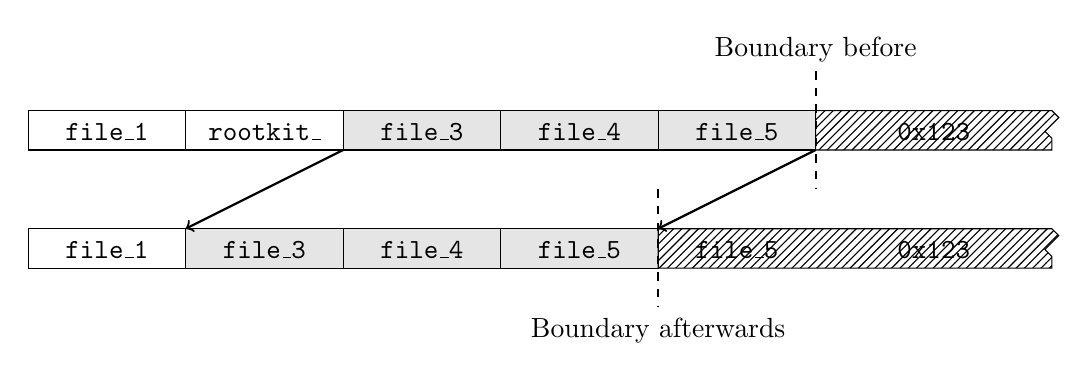
\begin{tikzpicture}
%% before
\foreach \x in {1,2} 
  \draw [draw=black] (\x*2,0) rectangle (\x*2+2,0.5);
\node at (5,0) [above] {\texttt{rootkit\_}};
\foreach \x in {3,4,5} 
  \draw [draw=black, fill opacity=0.1, fill=black] (\x*2,0) rectangle (\x*2+2,0.5);
\foreach \x in {1,3,4,5}
  \node at (\x*2 + 1, 0) [above] {\texttt{file\_\x}};
\draw (12, 0.5) -- (15, 0.5) [snake=zigzag, pattern = north east lines] -- (15, 0) [snake=none]-- (12,0) -- (12, 0.5);
\node at (13.5, 0) [above] {\texttt{0x123}};
\draw (12, 1)[above] node {Boundary before} [dashed, thick] -- (12, -0.5);
%% afterwards
\foreach \x in {1} 
  \draw [draw=black] (\x*2,-1) rectangle (\x*2+2,-1.5);
\foreach \x in {3,4,5} 
  \draw [draw=black, fill opacity=0.1, fill=black] (\x*2-2,-1) rectangle (\x*2,-1.5);
\foreach \x in {3,4,5}
  \node at (\x*2 - 1, -1.5) [above] {\texttt{file\_\x}};
\node at (3, -1.5) [above] {\texttt{file\_1}};
\node at (11, -1.5) [above] {\texttt{file\_5}};
\draw (10, -1) -- (15, -1) [snake=zigzag, pattern = north east lines] -- (15, -1.5) [snake=none]-- (10,-1.5) -- (10, -1);
\node at (13.5, -1.5) [above] {\texttt{0x123}};
\draw (10, -0.5) [dashed, thick] -- (10, -2) [below] node {Boundary afterwards};
%% arrows
\draw [->, draw=black, thick] (6,0) -- (4, -1);
\draw [->, draw=black, thick] (12,0) -- (10, -1);
\end{tikzpicture}
\caption{Hiding files by overwriting the file to be hidden and adjusting the number of returned bytes}
\label{fig:filehiding}
\end{figure}

Note that \texttt{getdents64} is the function that is called in most of the cases.
We tested \texttt{getdents} using a test program (testprogram.c).

Another implementation alternative would have been to manipulate the element preceeding the respective entries, such that it 
appears to be longer and thus kind of shades the item beginning with \textit{rootkit\_}.
This is done by modifying \texttt{d\_reclen} accordingly.

\subsection{Process Hiding}
Currently, we hook the readdir call of the proc-filesystem to hide the specified
tasks (just as in \autoref{filehiding}).

Another way to hide processes is to remove the respective task from the hash table 
which is used for looking up the tasks and generating the entries in proc.

\subsection{Module Hiding}
To hide the module, we 
\begin{itemize}
 \item remove it from the list of modules and
 \item hook the \texttt{readdir} operation of the sysfs.
\end{itemize}

The first point is pretty straightforward, once you have the pointer to the list of modules.
For the second one, you have to hook also create a \texttt{filldir}-function which gets called by the hooked readdir operation and returns 0 when called with this module as parameter.

\subsection{Socket Hiding}
Hiding sockets means that they are not displayed by neither netstat nor ss.
Netstat gets all its information through \texttt{/proc}, ss gets the tcp-socket information through the NETLINK interface of the kernel (when this is available), the udp information is also from \texttt{/proc}.
We implement socket hiding by hooking the \texttt{show}-operation of the seq\_file interface (only of tcp and udp socket-files in \texttt{/proc/net}, of course). Therefore We look at the port and the protocol of the passed \texttt{struct socket} and compare it with the socket to hide.

For tcp sockets displayed by ss, we hook the socketcall and return an error code when it gets called with a special combination of parameters. This lets ss also use its fallback alternative, which is \texttt{/proc} as already described.
\subsection{Privilege Escalation}

Privilege escalation is done using a simple mechanism: We set the user id of the current process to 0 (which corresponds to user \texttt{root}). This is done by the following code snippet\footnote{Note that these lines are just the central part of the \texttt{escalate} method.}:

\begin{verbatim}
void escalate(void){
    struct cred *my_cred;
    my_cred = prepare_creds(); 
    my_cred->uid = my_cred->euid = my_cred->suid = my_cred->fsuid = 0;
    my_cred->gid = my_cred->egid = my_cred->sgid = my_cred->fsgid = 0;
    commit_creds(my_cred);
}
\end{verbatim}

The function \texttt{prepare\_creds} creates a copy of the current threads credentials (i.e. user id, etc). We work on this copy (stored in \texttt{my\_cred}), and -- after modifying it -- apply the changes using \texttt{commit\_cred}.

While one could think it would be more convenient to directly modify the task's credentials, this is explicitly discouraged in the linux source code\footnote{File \texttt{kernel/cred.c}}.

\subsection{Covert Communication}
We hook \texttt{sys\_read} and intercept all input from standard in. 

First, we try to match a magic activating command. After this command, we read until a whitespace occurs. After that, we analyze what has been entered and execute the corresponding command, if 
\begin{itemize}
 \item it is available and
 \item it does not expect an argument.
\end{itemize}

If it does expect an argument (this is always a number), we read again until a whitespace and call the function with the parsed number as argument.

\end{document}
